\chapter{MIRI: The Mid-Infrared Instrument}
MIRI is an instrument that will provide unique capabilities for studying exoplanets and other cold and distant objects. This chapter will provide a detailed overview of the technical details and capabilities of the instrument. A complete description of MIRI is provided in a series of papers from \parencite{MIRI1,MIRI2,MIRI3, MIRI4,MIRI5,MIRI6,MIRI7,MIRI8,MIRI9}.
%MIRI is an imaging and spectroscopic instrument on board the James Webb Space Telescope (JWST). 
%
%
\section{The James Webb Space Telescope}
JWST is a 6.5 m space based observatory built in collaboration between NASA, ESA and CSA that will be located in a halo orbit at the L2 Earth-Sun Lagrange point. 
As the successor to the Hubble Space Telescope and the Spitzer Space Telescope, it will provide a new perspective for infrared astronomy. 
It is currently scheduled to launch in March 2021.

James Webb is fully optimized for infrared astronomy. 
To reduce instrumental thermal background, the entire telescope will operate at cryogenic temperatures. 
A large sun-shield will help block solar infrared radiation.
The lightweight beryllium mirrors are coated in gold to maximize reflectivity out to the mid infrared.

Of key interest to exoplanet science is the both the sensitivity and spatial resolution of the instrument. 
With its 6.5 m primary, JWST will have a spatial resolution from 0.01" at 0.6 micron to 0.92" at 29 micron.
The increase in sensitivity is due in part to the larger collecting area, but also to advances in detector technology since the previous generation of infrared observatories.
For example, the MIRI instrument will have a minimum detectable flux of 0.13 $\mu$Jy at 5.6 micron and a 10 000 second integration, or roughly a factor of 1000 better than what was possible with the Spitzer Space Telescope \parencite{MIRI9}.
\begin{figure}[t]
	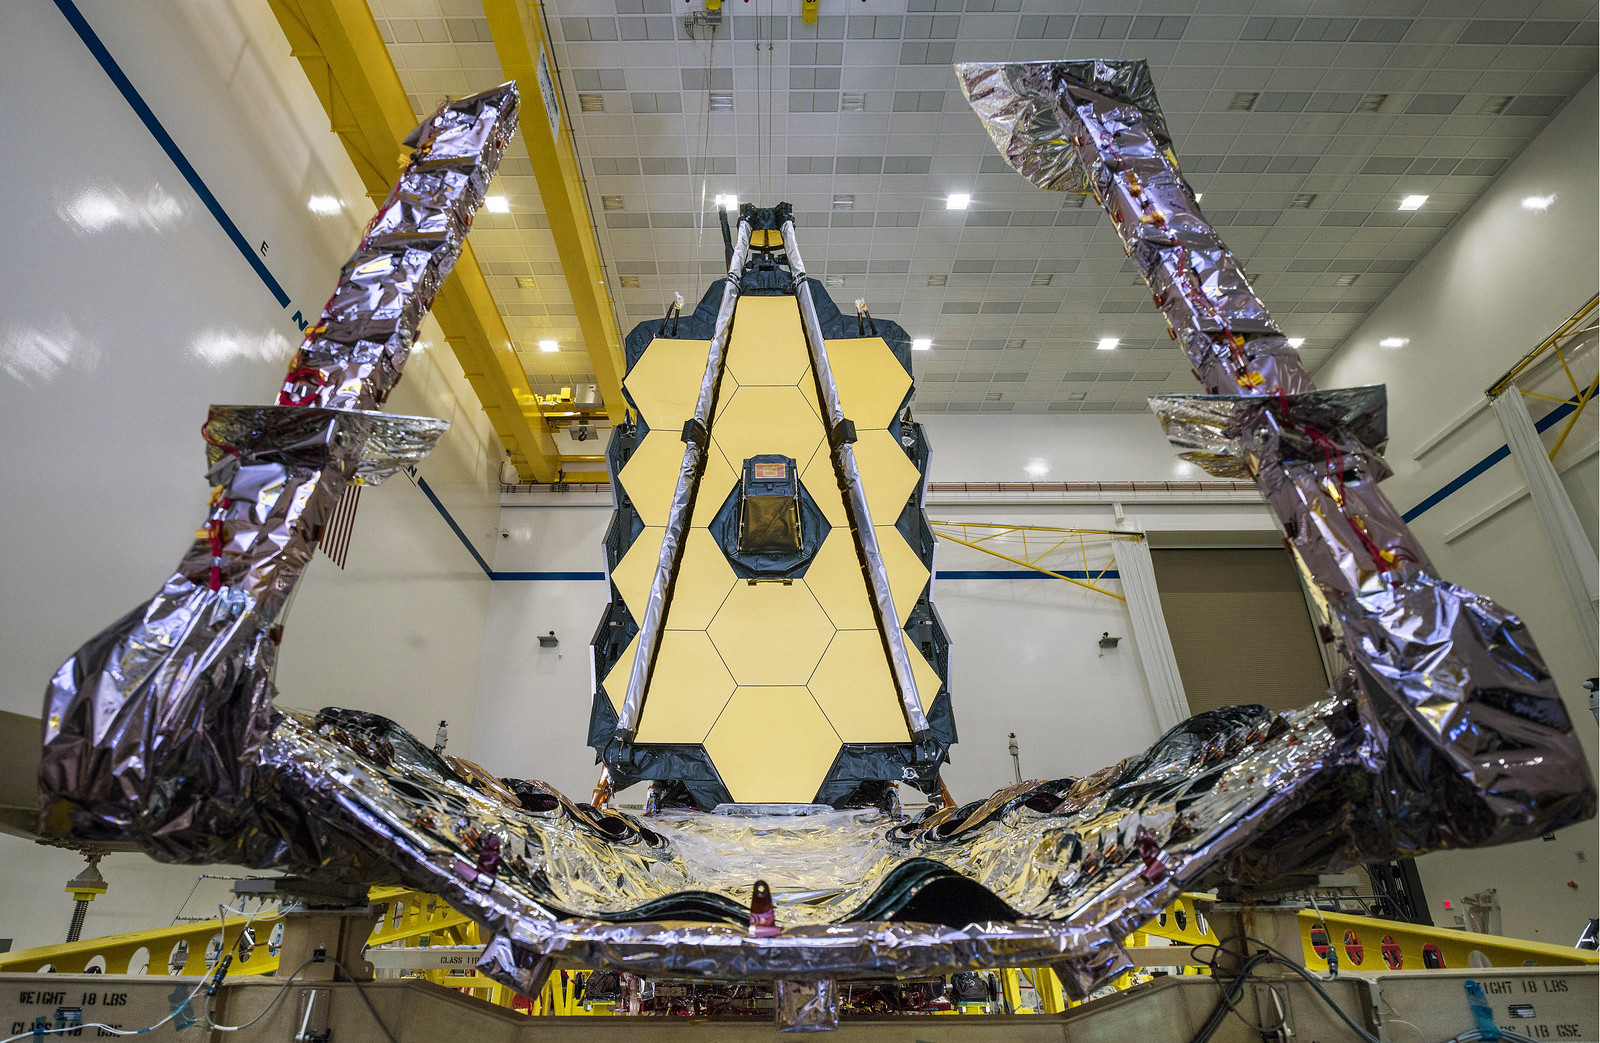
\includegraphics[width=\linewidth]{assembled.jpg}
	\caption{The James Webb Space Telescope during integration of the telescope into the Spacecraft Element \parencite{assembled}. }
	\label{fig:jwst}
\end{figure}

There are four primary instruments that constitute the Integrated Science Instrument Module (ISIM). 
Near-Infrared Camera (NIRCam), which provides imaging with coronagraphic capabilities from 0.6-5 micron.
The Near-Infrared Spectrograph (NIRSpec) provides fixed slit and integrated field unit spectroscopy capable of analyzing multiple objects simultaneously, and operates in the same wavelength range as NIRCam.
The Fine Guidance Sensor/ Near-Infrared Imager and Slitless Spectrograph (FGS/NIRISS) allows for low and medium resolution spectroscopy with high photometric stability, as well as aperture masking interferometry. 
The final instrument, MIRI, is the subject of this thesis.

\section{MIRI}
The Mid-Infrared Instrument (MIRI) provides imaging, fixed slit and integrated field spectroscopy between 4.8 and 28 micron \parencite{MIRI2}.
These sub-instruments are enclosed in a closed-cycle cooler to maintain a temperature of 6.7 K in order to reduce the thermal background.
At its most sensitive, MIRI is about 1000$\times$ more sensitive than comparable instrumentation on Spitzer. 
Sub-instrument sensitivities are shown in Fig. \ref{fig:sensitivities}.
While this will prove tremendously valuable for exoplanet science, it will also allow exploration of star formation, extra galactic astronomy and high-redshift observations. 
These and further science cases are described in \parencite{MIRI1}. 
In its imaging mode, MIRI can operate with either a Lyot or 4-Quadrant-Phase-Mask coronagraph to reduce stellar glare, the MRS is not equipped with such an element. 
Thus its use for exoplanet observations is restricted to highly separated or bright targets. 
It may also be possible to use the differences between the host star and companion spectra in order to image close in planets.

 %MIRI intro

\begin{table}[t]
	\begin{footnotesize}
	\centering
	\begin{tabular}{l|lll}
		\toprule
		\textbf{Subsystem} & \textbf{$\lambda$ Range [$\mu$m]} & \textbf{Px Scale ["/px]} & $\Delta\lambda/\lambda$\\
		\midrule
		Imaging & 5-28 & 0.11 & 3.5-16.1\\
		4QPM Coronagraphic Imaging & 10.65,11.4,15.5 & 0.11 & 14.1-17.2\\
		Lyot Coronagraphic Imaging & 23 & 0.11 & 4.1\\
		Low Resolution Spectroscopy & 5-12 & 0.11 & 100 @ 7.5$\mu$m\\
		Medium Resolution Spectroscopy & 4.9-28.8 & 0.196-0.273 & 1550-3300 \\
		\bottomrule
	\end{tabular}
	\caption{Summary of MIRI observing modes.}
	\label{tab:mirimodes}
	\end{footnotesize}
\end{table}
\begin{figure}[h]
	\centering
	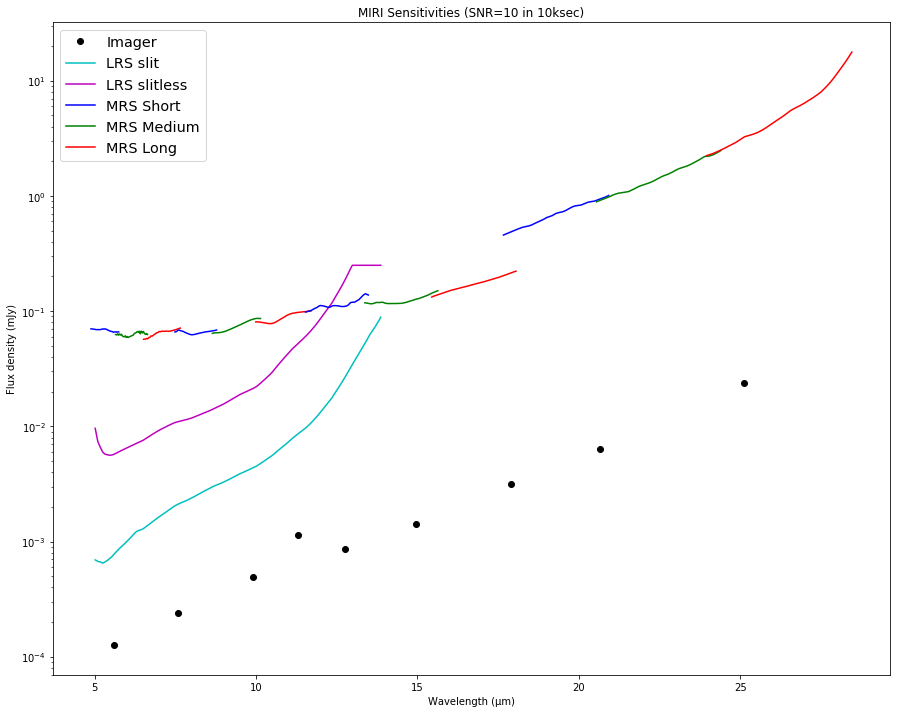
\includegraphics[width=0.8\linewidth]{mirisensitivities.png}
	\caption{Sensitivities of MIRI sub-instruments for an SNR of 10, with a 10 000s integration \parencite{MIRI1}.}
	\label{fig:sensitivities}
\end{figure}
\section{The Medium Resolution Spectrograph}\label{sec:mrs}
The Medium Resolution Spectrograph (MRS) consists of four integrated field spectrographs projected onto two detectors, covering 4.8-28 micron with a spectral resolution varying from R=1700 to R=3500.
Its FoV ranges from 4"$\times$4" to 7.7"$\times$7.7".
While a full description of the MRS is given in \parencite{MIRI6}, in this section we will outline the optical design of the instrument.
\begin{table}[t]
	\begin{small}
	\centering
	\begin{tabular}{l|lc|cccc}
		\toprule
		\textbf{Channel} & \textbf{Sub-band} & \textbf{Band} & \textbf{Detector} & $\lambda$ \textbf{Range [$\mu$m]} & \textbf{FoV [as]} & $\lambda$/$\Delta\lambda$\\
		\midrule
		\multirow{3}{*}{1}  &Short & 1A & \multirow{3}{*}{SW}   & 4.83 - 5.82 & 3.46$\times$3.72 & 3500 \\
							&Medium & 1B &						& 5.62 - 6.73 & 3.46$\times$3.72 & 3500 \\
							& Long & 1C&						& 6.46 - 7.76 & 3.41$\times$3.72 & 3300 \\
		\midrule
		\multirow{3}{*}{2}  &Short & 2A & \multirow{3}{*}{SW}   & 7.44 - 8.90 & 4.16$\times$4.76 & 3000 \\
							&Medium & 2B &						& 8.61 - 10.28 & 4.16$\times$4.76 & 3000 \\
							& Long & 2C&						& 9.94 - 11.87 & 4.12$\times$4.76 & 3000 \\
		\midrule
		\multirow{3}{*}{3}  &Short & 3A & \multirow{3}{*}{LW}   & 11.47 - 13.67 & 6.00$\times$6.24 & 2700 \\
							&Medium & 3B &						& 13.25 - 15.80 & 5.96$\times$6.24 & 2300 \\
							& Long & 3C&						& 15.30 - 18.24 & 5.91$\times$6.24 & 2300 \\		
		\midrule
		\multirow{3}{*}{4}  &Short & 3A & \multirow{3}{*}{LW}   & 17.54 - 21.10 & 7.14$\times$7.87 & 1700 \\
							&Medium & 3B &						& 20.44 - 24.72 & 7.06$\times$7.06 & 1700 \\
							& Long & 3C&						& 23.84 - 28.82 & 6.99$\times$7.87 & 1500 \\			
		\bottomrule
	\end{tabular}
	\end{small}
	\caption{Properties of the MIRI MRS channels \parencite{MIRI6}.}
	\label{tab:mrs}
\end{table}

\subsection{Coordinates}
There are three primary coordinate systems in use with JWST/MIRI-MRS, of which two will be relevant for this thesis, with the detector and local MRS coordinates described in Fig. \ref{fig:mrscoords} \parencite{Argyriou2020}.

The detector coordinate grid is formed by counting x/y pixels, as well as the slice number.
Each of the two MRS detectors is an array of 1032$\times$1024 pixels, though only 1024 are photosensitive in the horizontal direction.
Each image slice from the IFU appears as a curved stripe on the detector, though neighboring stripes on the detector do not correspond to neighbouring slices of the image. 

The local MRS coordinate system is described in terms of $\alpha,\beta$ and $\lambda$. The continuous $\alpha$ coordinate is the along slice direction, while $\beta$ is perpendicular and discrete, corresponding to the slice number. $\lambda$ is the wavelength. Both $\alpha$ and $\lambda$ are fit by a second order polynomial to account for along and across slice distortion \parencite{MIRI6}. Each detector sub array has its own mapping to $\alpha,\beta,\lambda$ space, due to the differences in FoV, slice count, distortion and spectral resolution.

The third coordinate frame is the global coordinate system of JWST itself, V1,V2,V3. The V1 coordinate refers to the symmetry axis of the telescope, V3 points towards the foldable secondary mirror support structure strut. V2 completes the coordinate system, being orthogonal to V1 and V3. This coordinate system will not be used in this thesis.

\begin{figure}[t]
	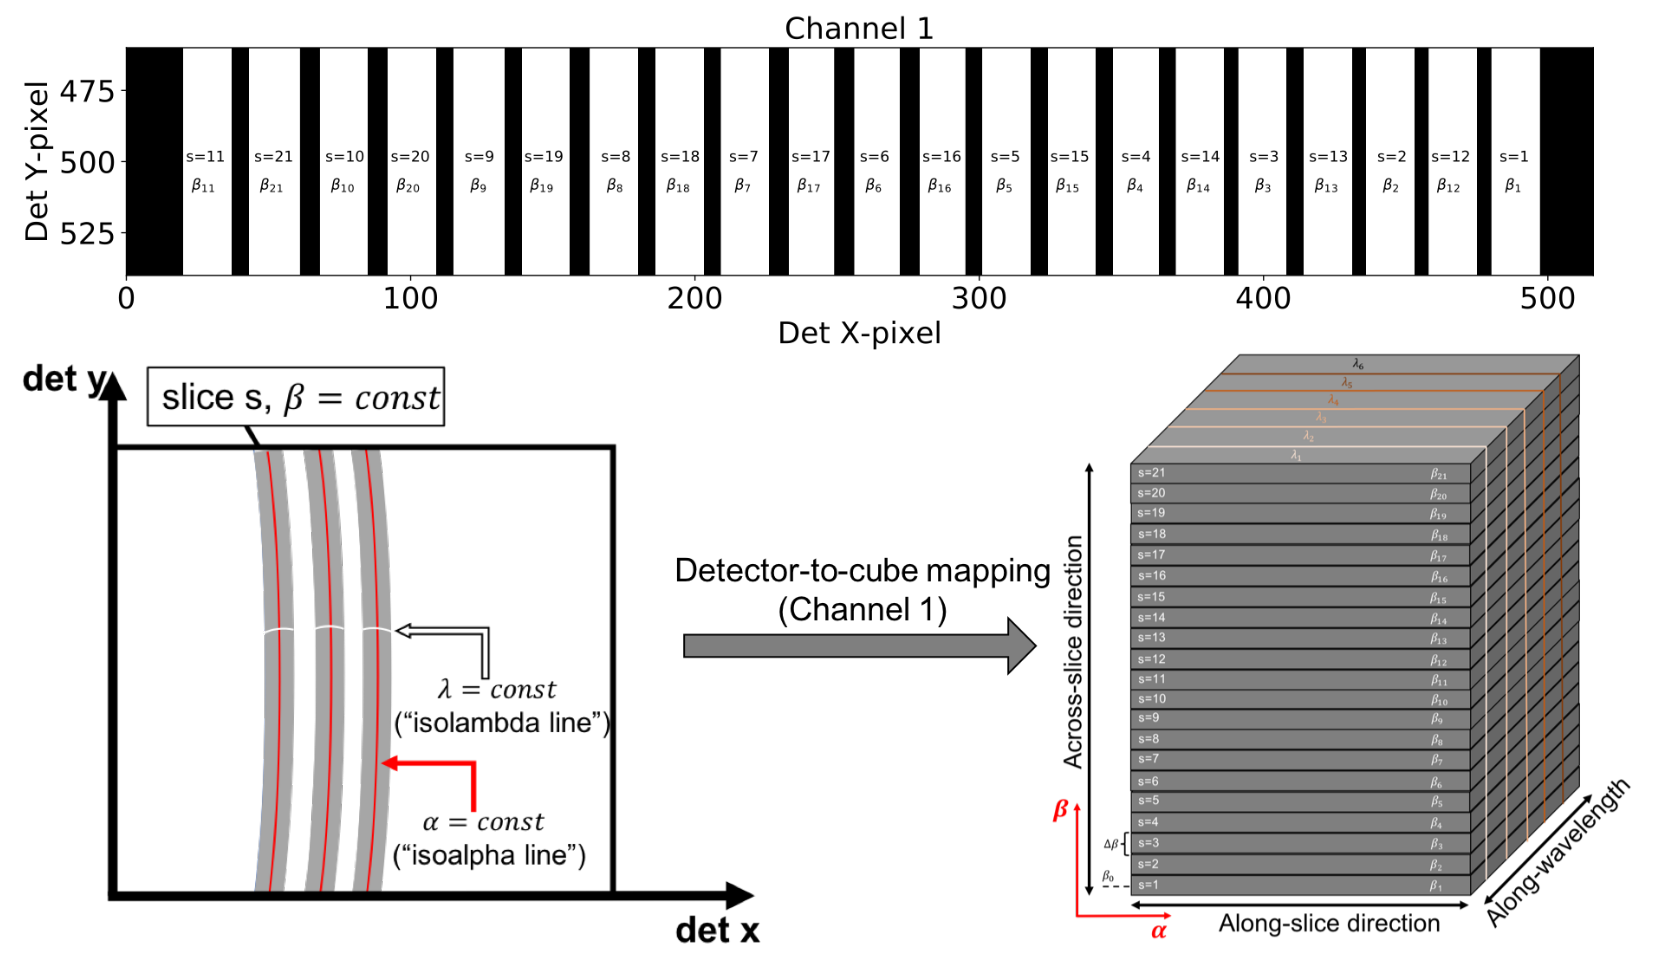
\includegraphics[width=\linewidth]{coordinates.png}
	\caption{Description of the MRS detector (x,y,s) coordinate system to the local MRS ($\alpha,\beta,\lambda$) cube coordinates. \textbf{Top}: Detector coordinates. Note that the consecutive stripe numbers s$_{i}$, s$_{i+1}$ correspond to neighbouring image slices. \textbf{Bottom}: Description of the (invertible) detector-to-cube transformation \parencite{Argyriou2020}.}
	\label{fig:mrscoords}	
\end{figure}

\begin{figure}[t]
	\centering
	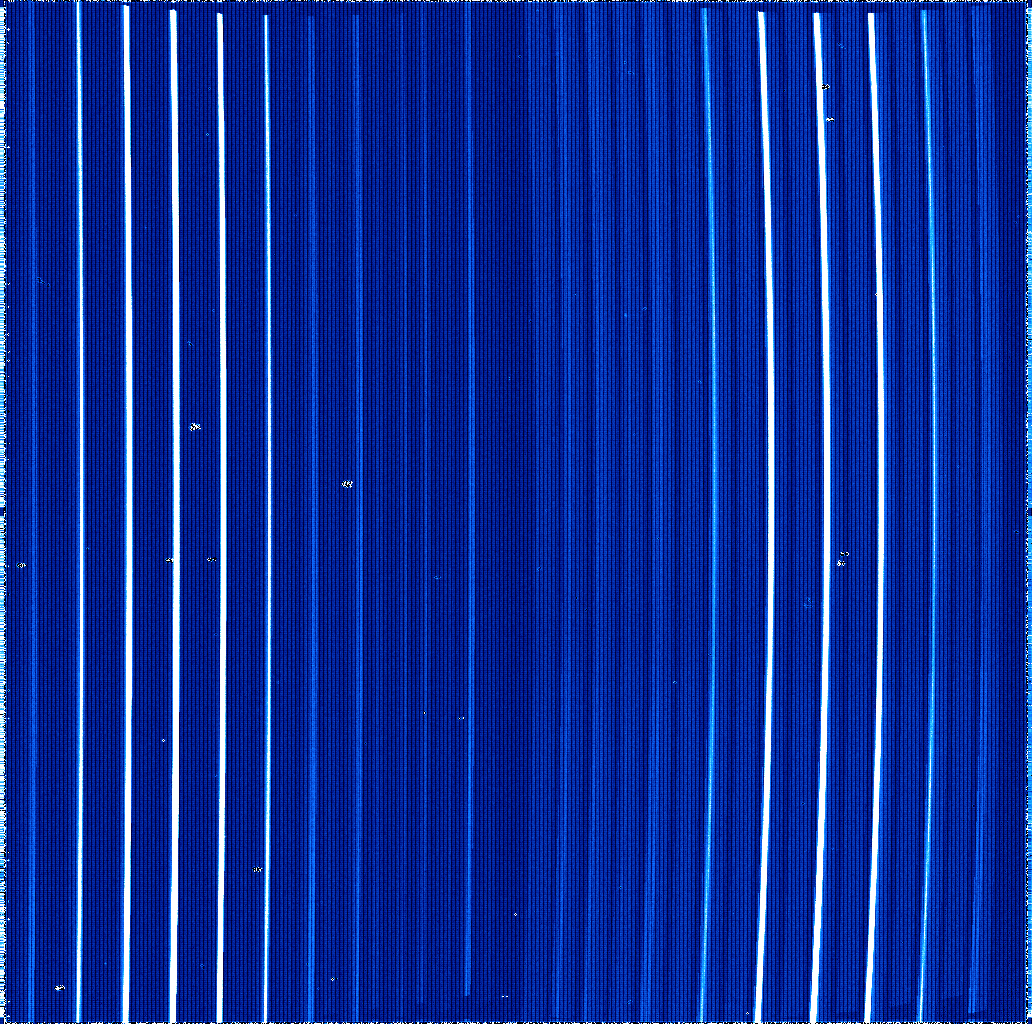
\includegraphics[width = 0.45\linewidth]{MRSRAW.png}
	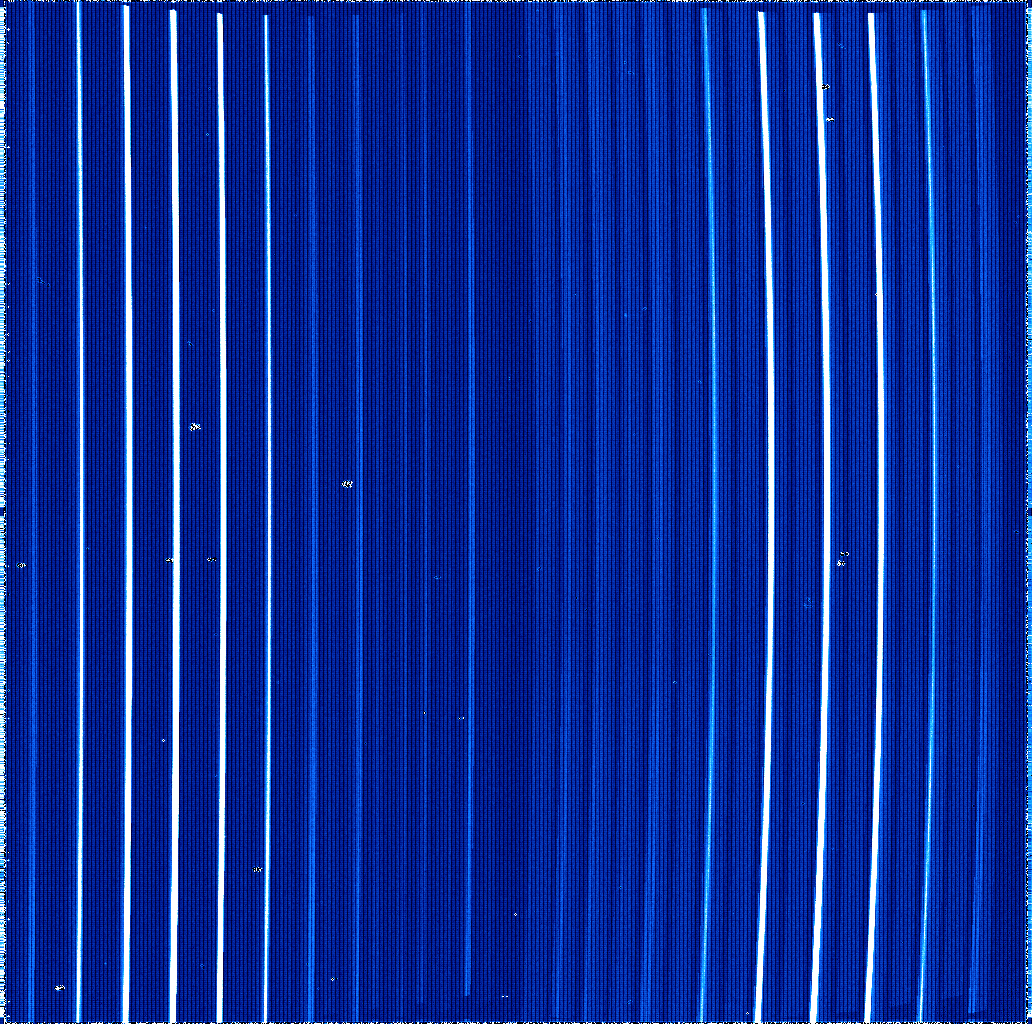
\includegraphics[width = 0.45\linewidth]{MRSRAW.png}
	\caption{Detector images of a spatially and spectrally flat calibration source for the SW detector (left) and LW detector (right). FIXMEREPLACE}
	\label{fig:flatfield}
\end{figure}
\subsection{Integral Field Spectroscopy}
\begin{wrapfigure}{r}{5.5cm}
	\vspace{-1em}
	
\includegraphics[width=5.5cm]{WISE0855_Dither_Cube_1A.png}
	\caption{The reconstructed JWST PSF as imaged by the MRS, using a 2-pattern dither.}
	\label{fig:miripsf}
\end{wrapfigure}
As an integrated field spectrograph (IFS) consisting of 4 integrated field units (IFUs), the MRS provides both spatial and spectral information.
This is accomplished by slicing the on sky image, and performing spectroscopy on each of the image slices. 
Here we will step step through some of the key optical systems used to accomplish this, while a more detailed description of the optics is given in section 2 of \parencite{MIRI6}.

A series of optics picks off a FoV from the telescope beam, and directs it to the IFU slicing mirrors, where the focal plane is re-imaged. 
The image slicer consists of an array of thin mirrors at unique angles, in order to separate different spatial slices of the on-sky image.
The across slice width is equal to the FWHM of the Airy pattern at the shortest wavelength of the given IFU.
There are a total of 4 image slicers, one for each of the MRS channels.
Each slice is then collimated, and directed to a diffraction grating. 
Each channel has 3 separate gratings, each covering approximately a third of the wavelength range of each channel. 
Thus it requires 3 total exposures to cover the wavelength range of a channel.
Channels 1 and 2 are each projected onto separate halves of a single detector, as are channels 3 and 4 as seen in Fig. \ref{fig:flatfield}.
When reconstructed, the PSF is an undersampled image of the JWST PSF, though dithering can be used to improve the spatial sampling.
As such, multiple wavelength ranges are imaged simultaneously, and it requires only 3 exposures in order to cover the entire MRS wavelength range. 
\subsection{Detectors}
MIRI uses three arsenic-doped silicon (Si:As) impurity band conduction (IBC) detectors descended from those used in the Spitzer Space Telescope.
Each detector uses a 1024$\times$1024 pixel format.
One detector is used for the imaging and LRS modes, while the remaining two detectors are used in the MRS.
The full technical details of the detectors are described in \parencite{MIRI7}.

Si:As IBC detectors are ideal for mid-infrared measurements.
Each detector is built onto a high resistivity transparent contact. 
A 25-35 micron thick, heavily arsenic doped layer acts as the absorption layer, with an electric field maintained across the layer in order to transport the generated photoelectron.
A transparent contact layer provides a connection to the detector electronics, where the signal is amplified and read out.
A schematic of the layers in the detector is provided in the context of the fringing effect in Fig. \ref{fig:layers}.
These detectors have a quantum efficiency that is wavelength dependent, and provides a fundamental limitation on the sensitivity.
Precise measurement of this photon-to-electron conversion efficiency is critical for photometrically calibrating observations. 
The efficiencies are shown for each sub-band of the MRS detectors in Fig. \ref{fig:mirideteff}.
\begin{figure}[t]
	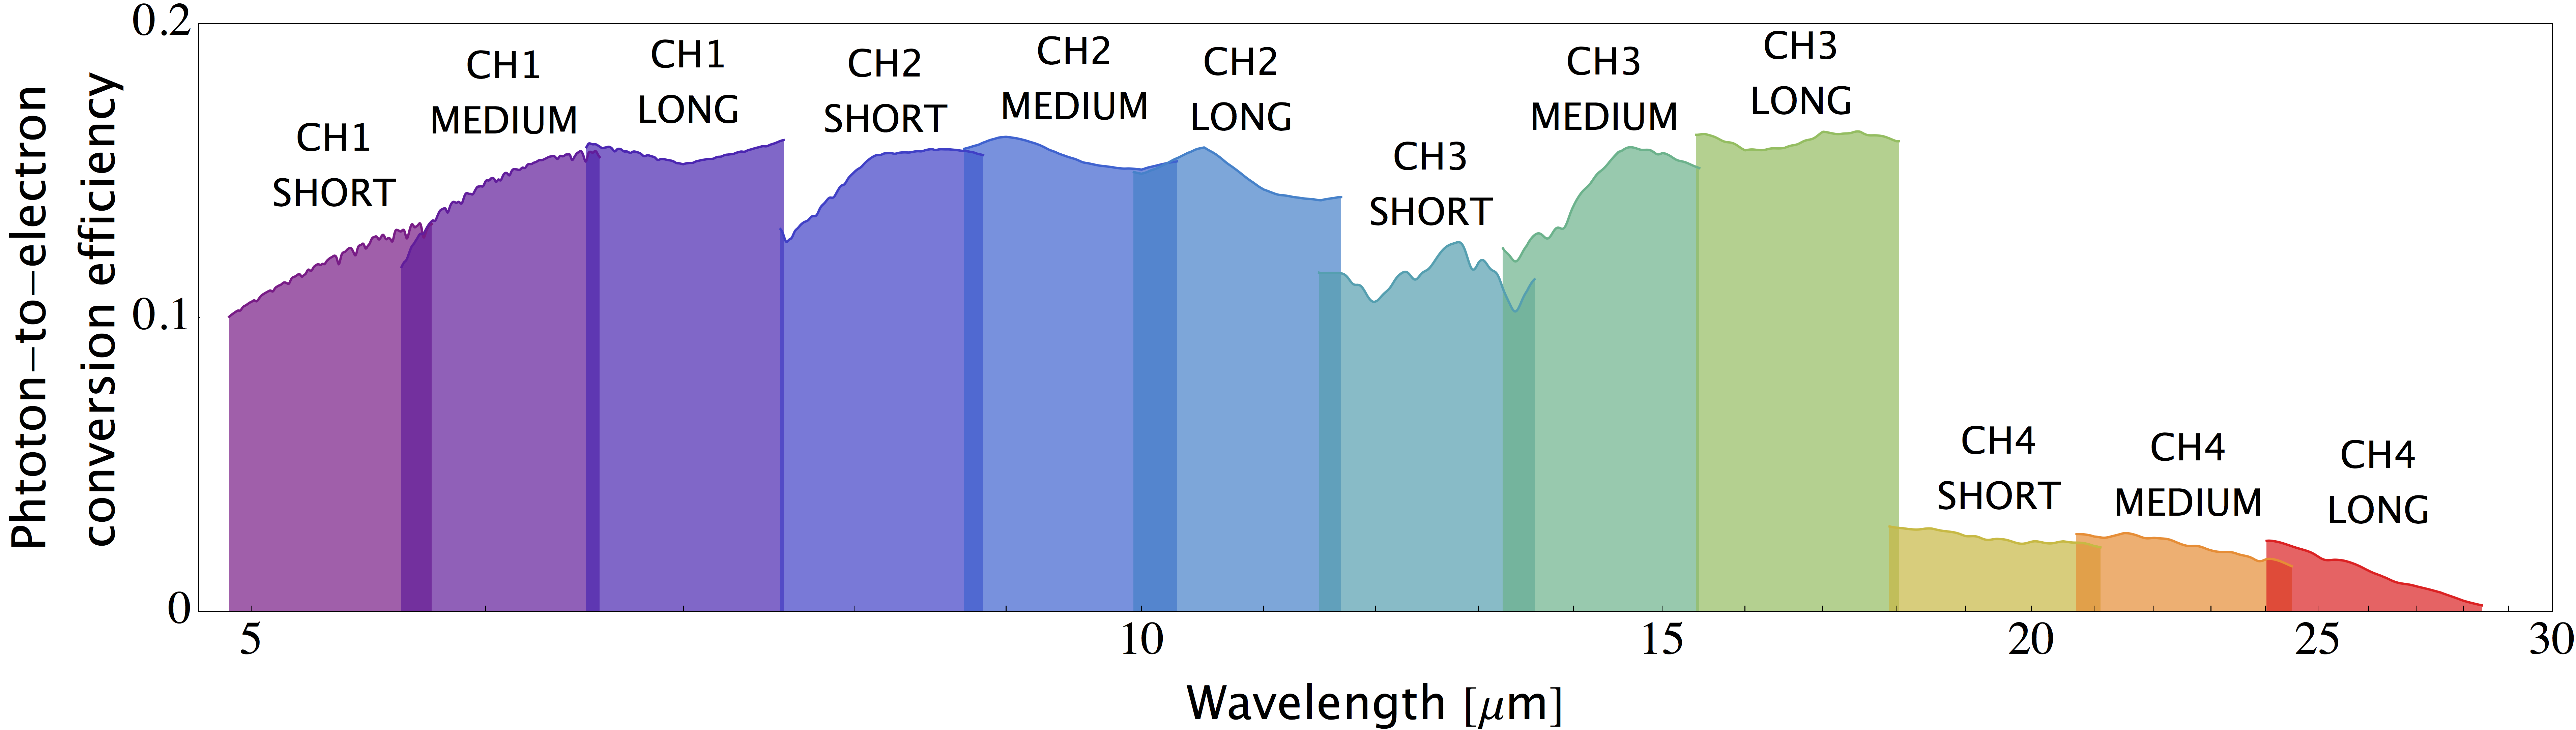
\includegraphics[width=\linewidth]{MIRI_MRS2.png}
	\caption{Average photon-to-electron conversion efficiencies for the MIRI MRS detectors.}
	\label{fig:mirideteff}
\end{figure}
\subsubsection{Readout Modes}
The MRS has two primary readout modes, which can be selected for different observing strategies.
\begin{itemize}
	\item FAST - A 2.78 s integration with a single sample per pixel. Higher noise, but more suited for bright targets.
	\item SLOW - a 24 s integration, with 9 samples per pixel. A lower noise mode, but can saturate on bright sources.
\end{itemize}

\section{Observations}
The observations in this work are based on proposed exoplanet observations for the ERS and GTO programs.
The observing parameters have been checked using the JWST Exposure Time Calculator in order to ensure sufficient SNR.
Several of the observations make use of a dithering procedure, described below.
\subsection{Dithering}
The MIRI PSF is spatially undersampled in the MRS in order to allow for wider wavelength coverage and increased throughput.
This design choice was made in order to reduce the weight of components that would be necessary in order to provide a fully sampled PSF while meeting the spectroscopic requirements.
In order to fully sample the PSF, observations are dithered: that is, multiple telescope pointings are used, and the exposures from each pointing combined into a single observation.
An optimal dithering strategy for each channel has been designed in order to fully sample the PSF in a minimum of observations. 
For a point source, it will be typical to use a 2 or 4 point dither pattern.

\subsection{Exposure time calculations}
The JWST Exposure time calculator (ETC) is a publicly available tool that can be used to estimate outcomes of a given set of observational parameters on a specified target.
This can be used to estimate the SNR in different wavelength bands, optimize observing  and check for detector saturation.
All observations in this work were checked using the ETC in order to prevent saturation and ensure sufficient SNR.
However, we did not attempt to optimize the observing strategy for our targets, and instead used the parameters specified in the ERS and GTO observing proposals.